\PassOptionsToPackage{table}{xcolor}
\documentclass{beamer}\usepackage[]{graphicx}\usepackage[]{color}
%% maxwidth is the original width if it is less than linewidth
%% otherwise use linewidth (to make sure the graphics do not exceed the margin)
\makeatletter
\def\maxwidth{ %
  \ifdim\Gin@nat@width>\linewidth
    \linewidth
  \else
    \Gin@nat@width
  \fi
}
\makeatother

\definecolor{fgcolor}{rgb}{0.345, 0.345, 0.345}
\newcommand{\hlnum}[1]{\textcolor[rgb]{0.686,0.059,0.569}{#1}}%
\newcommand{\hlstr}[1]{\textcolor[rgb]{0.192,0.494,0.8}{#1}}%
\newcommand{\hlcom}[1]{\textcolor[rgb]{0.678,0.584,0.686}{\textit{#1}}}%
\newcommand{\hlopt}[1]{\textcolor[rgb]{0,0,0}{#1}}%
\newcommand{\hlstd}[1]{\textcolor[rgb]{0.345,0.345,0.345}{#1}}%
\newcommand{\hlkwa}[1]{\textcolor[rgb]{0.161,0.373,0.58}{\textbf{#1}}}%
\newcommand{\hlkwb}[1]{\textcolor[rgb]{0.69,0.353,0.396}{#1}}%
\newcommand{\hlkwc}[1]{\textcolor[rgb]{0.333,0.667,0.333}{#1}}%
\newcommand{\hlkwd}[1]{\textcolor[rgb]{0.737,0.353,0.396}{\textbf{#1}}}%

\usepackage{framed}
\makeatletter
\newenvironment{kframe}{%
 \def\at@end@of@kframe{}%
 \ifinner\ifhmode%
  \def\at@end@of@kframe{\end{minipage}}%
  \begin{minipage}{\columnwidth}%
 \fi\fi%
 \def\FrameCommand##1{\hskip\@totalleftmargin \hskip-\fboxsep
 \colorbox{shadecolor}{##1}\hskip-\fboxsep
     % There is no \\@totalrightmargin, so:
     \hskip-\linewidth \hskip-\@totalleftmargin \hskip\columnwidth}%
 \MakeFramed {\advance\hsize-\width
   \@totalleftmargin\z@ \linewidth\hsize
   \@setminipage}}%
 {\par\unskip\endMakeFramed%
 \at@end@of@kframe}
\makeatother

\definecolor{shadecolor}{rgb}{.97, .97, .97}
\definecolor{messagecolor}{rgb}{0, 0, 0}
\definecolor{warningcolor}{rgb}{1, 0, 1}
\definecolor{errorcolor}{rgb}{1, 0, 0}
\newenvironment{knitrout}{}{} % an empty environment to be redefined in TeX

\usepackage{alltt}

\mode<presentation>
{
  \usetheme{Warsaw}
  
}

\beamertemplatenavigationsymbolsempty 

\usepackage[]{inputenc}
\usepackage[english]{babel}
\usepackage{amsthm}
\usepackage{graphicx}
\usepackage{epstopdf}
\usepackage{grffile}
\usepackage{hyperref}
\usepackage{beamerthemesplit}
\definecolor{links}{HTML}{2A1B81}
\hypersetup{colorlinks,linkcolor=,urlcolor=links}
%\setsansfont[Ligatures={Common,TeX}]{TeX Gyre Heros}

{\renewcommand{\arraystretch}{1.1}

\AtBeginSection[]
{
  \begin{frame}
    \frametitle{Outline}
    \tableofcontents[currentsection]
  \end{frame}
}

\newcommand*\oldmacro{}%
\let\oldmacro\insertshorttitle%
\renewcommand*\insertshorttitle{%
   \oldmacro\hfill%
   \insertframenumber\,/\,\inserttotalframenumber}

\setbeamertemplate{headline}{}
\setbeamertemplate{itemize items}[circle]
\title[Statistical analysis of an antibody repertoire]{Statistical analysis of full-length antibody repertoire using immunosequencing data}

\author [Andrew Bzikadze]{Andrew Bzikadze\\ \texttt{\small{\href{mailto:seryrzu@gmail.com}{seryrzu@gmail.com}}}}
%\institute{Saint Petersburg State University, Russia \\
%           Faculty of Mathematics and Mechanics \\
%           Department of Statistical Modelling}
\date {
September 13, 2015
}

\usepackage[absolute,overlay]{textpos}
\setlength{\TPHorizModule}{1cm} % Horizontale Einheit
\setlength{\TPVertModule}{1cm} % Vertikale Einheit
\addtobeamertemplate{title page}{
}{}
\IfFileExists{upquote.sty}{\usepackage{upquote}}{}

\begin{document}
\begin{frame}
  \titlepage
\end{frame}

\section{Introduction and Motivation}

\begin{frame}{Introduction: \texttt{V(D)J-recombination}}
  Immunoglobulin heavy chain locus:
  \begin{figure}[h]
    \center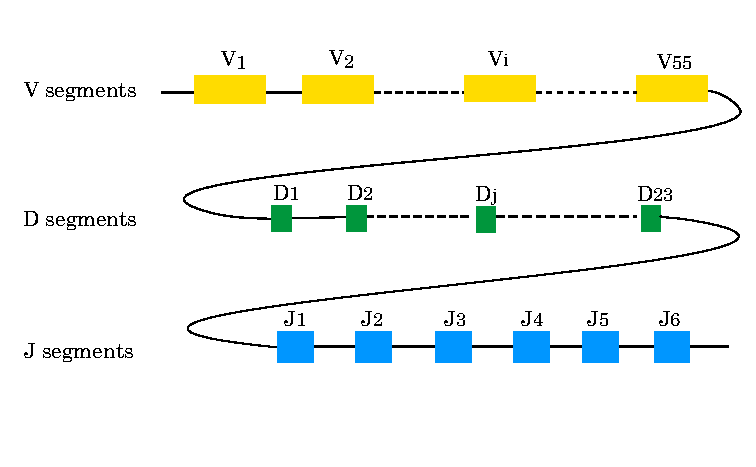
\includegraphics[width=300pt]{Pictures/vdj1.pdf}
 \end{figure}
\end{frame}

\begin{frame}{Introduction: \texttt{V(D)J-recombination}}
  Segment of each type is selected: 
  \begin{figure}[h]
    \center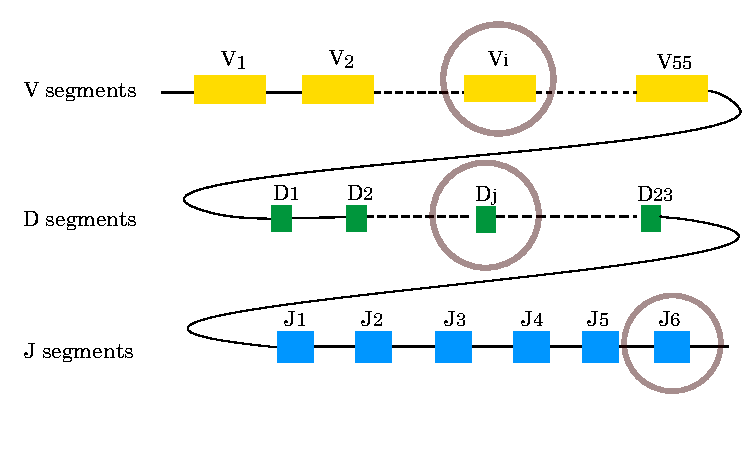
\includegraphics[width=300pt]{Pictures/vdj2_select_genes.pdf}
 \end{figure}
\end{frame}

\begin{frame}{Introduction: \texttt{V(D)J-recombination}}
  3 types of biochemical events: \textit{palindrome}, \textit{cleavage}, \textit{non-genomic insertion}. 
  \begin{figure}[h]
    \center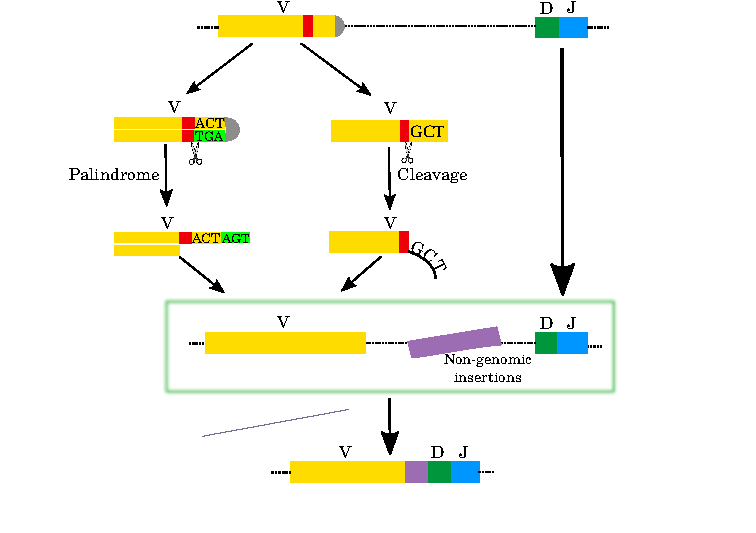
\includegraphics[width=300pt]{Pictures/vdj3_DJ_aligned_new.pdf}
 \end{figure}
\end{frame}

\begin{frame}{Introduction: \texttt{V(D)J-recombination}}
  Further optimization of antibody affinity is achieved through extensive mutations referred as \textit{somatic hypermutations}:
  \begin{figure}[h]
    \center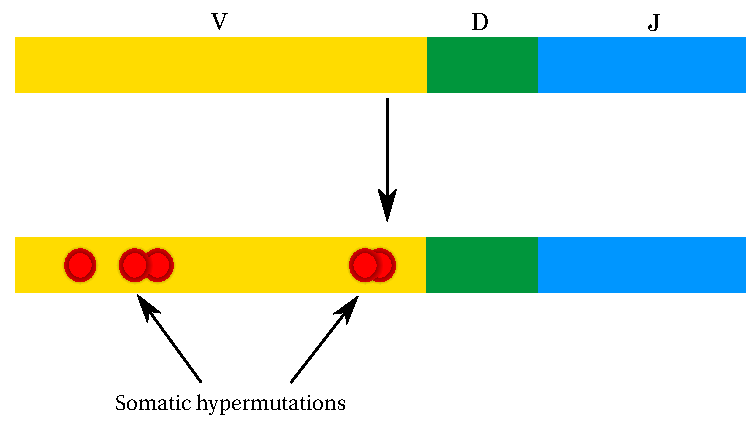
\includegraphics[width=300pt]{Pictures/somatic_mutations.pdf}
 \end{figure}
\end{frame}

\begin{frame}{Introduction: \texttt{V(D)J-recombination}}
  Because we do not know the deterministic nature of the \texttt{V(D)J-recombination}, it is reasonable
  to consider it as a {\color{blue} random} (stochastic) process.

  \bigskip
  Hence the analysis of somatic recombination can be done in statistical and simulation terms. 
\end{frame}

\begin{frame}{Motivation: comparing different antibody repertoires}
  \texttt{B}-cells:
  {\footnotesize
  \begin{itemize}
    \item \href{http://www.ncbi.nlm.nih.gov/pmc/articles/PMC1065207/}{Comparison of Antibody Repertoires against \texttt{Staphylococcus aureus} in 
      Healthy Individuals and in Acutely Infected Patients --- Agnieszka Dryla \textit{et al.}, CVI, 2005}.
  
    \item \href{http://www.ncbi.nlm.nih.gov/pubmed/9882391}{Comparison of the antibody repertoire generated in healthy volunteers following immunization with a monomeric recombinant \texttt{gp120} 
      construct derived from a \texttt{CCR5/CXCR4}-using human immunodeficiency virus type 1 isolate with sera from naturally infected individuals --- Beddows S. \textit{et al.}, Journal of Virology, 1999}. 
  \end{itemize}
  }

  \bigskip
  \texttt{T}-cells:
  
  { \footnotesize
  \begin{itemize}
    \item \href{http://www.ncbi.nlm.nih.gov/pubmed/26297792}{Donor Unrestricted \texttt{T} Cells: A Shared Human \texttt{T} Cell Response --- Van Rhijn I, Moody DB, Journal of Immunology, 2015}.
    \item \href{http://www.ncbi.nlm.nih.gov/pubmed/21349924}{Exhaustive \texttt{T}-cell repertoire sequencing of human peripheral blood samples reveals 
      signatures of antigen selection and a directly measured repertoire size of at least 1 million clonotypes --- Warren RL \textit{et al.}, Genome Research, 2011}.
  \end{itemize}
  }
  %\textbf{Motivation:} knowledge of the distribution of nucleotide sequences potentially helps with a lot of things.
  %\begin{itemize}
  %  \item Simulation of pair reads: improvements of \texttt{IgSimulator}.
  %  \item Dealing with Clonal Trees. ???
  %  \item Comparison of different antibody repertoires.
  %  \item String metrics for measuring the difference between two sequences: improvements of \texttt{IgRepertoireConstructor}.
  %\end{itemize}
\end{frame}

\begin{frame}{Motivation: simulation of a repertoire}
  Appropriate statistical model of somatic recombinations potentially improves \texttt{IgSimulator}, making it more ``realistic''.
  
  \begin{figure}[h]
    \center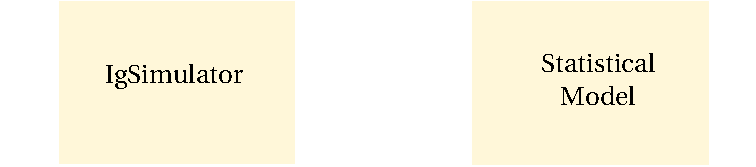
\includegraphics[width=300pt]{Pictures/igsimulator.pdf}
  \end{figure}
\end{frame}

\begin{frame}{Motivation: Clonal trees}
  Clear situation:
  \begin{figure}[h]
    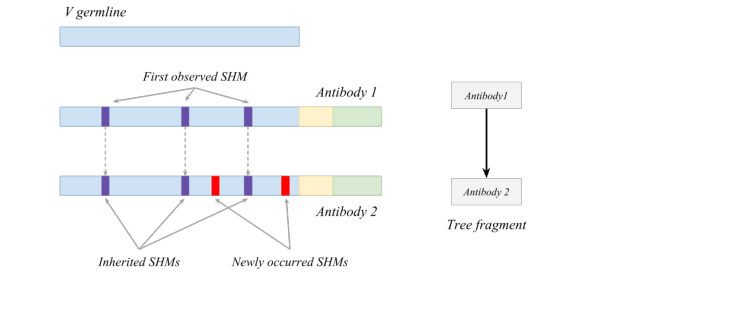
\includegraphics[width=400pt]{Pictures/clonal_trees1.pdf}
  \end{figure}
\end{frame}

\begin{frame}{Motivation: Clonal trees}
  Arguable situation:
  \begin{figure}[h]
    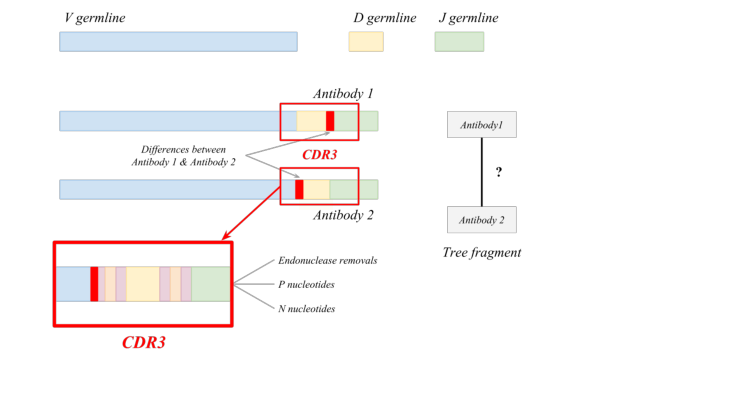
\includegraphics[width=400pt]{Pictures/clonal_trees2.pdf}
  \end{figure}
\end{frame}

\begin{frame}{Motivation: \texttt{IgRepertoireConstructor}}
  \begin{columns}[c]
    \begin{column}{0.5\textwidth}
      \begin{figure}[h]
        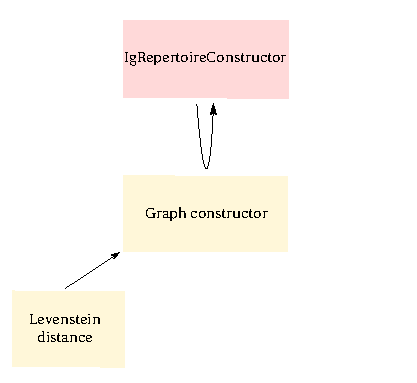
\includegraphics[width=200pt]{Pictures/igRepConstr1.pdf}
      \end{figure}
    \end{column}
    \begin{column}{0.4\textwidth}
      \begin{center}
        The current release of the \texttt{IgRepertoireConstructor} uses Levenstein distance to construct edges in the graph.
      \end{center}
    \end{column}
  \end{columns}
\end{frame}

\begin{frame}{Motivation: \texttt{IgRepertoireConstructor}}
  \begin{columns}[c]
    \begin{column}{0.5\textwidth}
      \begin{figure}[h]
        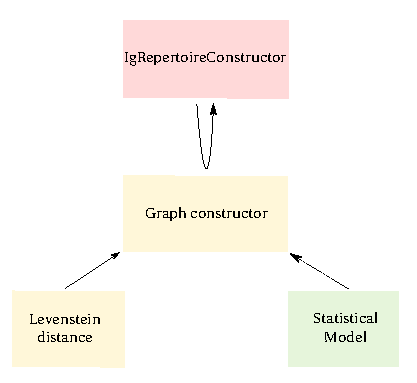
\includegraphics[width=200pt]{Pictures/igRepConstr2.pdf}
      \end{figure}
    \end{column}
    \begin{column}{0.4\textwidth}
      \begin{center}
        The statistical model could suggest a more delicate approach.
      \end{center}
    \end{column}
  \end{columns}
\end{frame}

%\begin{frame}{Introduction}
%  \textbf{Research direction:} analysis of input merged pair reads using statistical and simulation methods.
%  
%  \pause 
%  \textbf{Questions:}
%  \begin{itemize}
%    \item What is the distribution law of nucleotide subsequences of merged pair reads?
%    \item Is there any correlation between biological events (for instance, between \textit{cleavage} / \textit{palindromes} and specific gene segments)?
%    \item What model describes biological events the best (for example, \textit{non-genomic insertion} at the \texttt{VD}-, \texttt{DJ}- junction)? 
%  \end{itemize}
%\end{frame}

\begin{frame}{Tasks}
  There are plenty of tasks. To name a few:
  \begin{itemize}
    \item What is the correlation between \texttt{D-J} and \texttt{V-DJ} joining?
    \item Is there any correlation between the \textit{cleavage} / \textit{palindromes} and specific gene segments?  
    \item What are the properties of the \textit{non-genomic insertion}?
  \end{itemize}
\end{frame}

\begin{frame}{Background}
  An article about the distribution law of \texttt{CDR3} generating recombinations for \texttt{T}-cells:
  
  \href{http://www.pnas.org/content/109/40/16161.full}{%Statistical inference of the generation probability of \texttt{T}-cell receptors from sequence repertoires (
  Anand Murugana, Thierry Morab, Aleksandra M. Walczakc and Curtis G. Callan --- 2012}:
  \begin{itemize}
    \item Analysis is focused on non-productive \texttt{CDR3}s.
    \item Suggested model sets joint distribution over the set of discrete variables: \textit{identities} of \texttt{V-, D-, J-} genes, number of \textit{deletions} from the end of a segment, \textit{palindromic} nucleotides and \textit{non-genomic insertion} at the end of a gene.
    \pause
  \item {\color{blue} 2865(!) parameters to estimate.}
  \end{itemize}
\end{frame}

\begin{frame}{Background}
  \textbf{Questions about the paper:}
  \begin{itemize}
    \item Is the suggested model really adequate (including the problem of potential overfitting)?
    \item Are the results statistically significant?
    \item Are similar results true for \texttt{B}-cells?
  \end{itemize}
% 
%  \pause
%  \bigskip
%  {\color{blue} Difficult to answer, should start with something simpler.}
\end{frame}

\begin{frame}{Two types of events}
 % It is reasonable to classify events (palindromes, cleavage, etc.) into ``{\color{blue} biological}'' and ``{\color{blue} accidental}''.
  

  The goals 
  \begin{itemize}
    \item correlations between \textit{palindromes} and specific gene segments,
    \item properties of the \textit{non-genomic insertion}
  \end{itemize}
  include the task of distinguishing {\color{blue} ``biological''} (meaningful) events from {\color{blue} ``accidental''} (random) observations and hence require additional knowledge about repertoire structure.
  
  \bigskip
  Considering that first we decided to concentrate on a problem of computation of correlation between \textbf{cleavage and specific gene segments}.
 
  \pause
  \bigskip
  {\color{blue} Unlike two problems above \textit{cleavage} can always be detected precisely according to the alignment.}
\end{frame}

\section{Cleavage and specific gene segments}
\begin{frame}{Cleavage and specific gene segments}

Antibody repertoire is a result of V(D)J recombination and secondary diversification. To analyze properties of V(D)J recombination only we perform the following steps:
 
  \pause
  %\textbf{Idea:} Let's take only genes, that align to the germline with  level at least $C$, where $0 \leqslant C \leqslant 1$.
  \bigskip 
  \small{
  \begin{columns}[T]
    \begin{column}{0.6\textwidth}
      \begin{itemize}
        \item Constuct a full-length antibody repertoire using \texttt{IgRepertoireConstructor}.
        \item Consider {\color{blue} highly abundant antibody clusters} of the constructed repertoire.
        \item Apply \texttt{IgBlast} to reads corresponding to selected clusters.
        \item To avoid effects of the secondary diversification filter out reads with \textit{low} alignment score.
      \end{itemize}
    \end{column}
    \begin{column}{0.5\textwidth}
      \begin{figure}[h]
        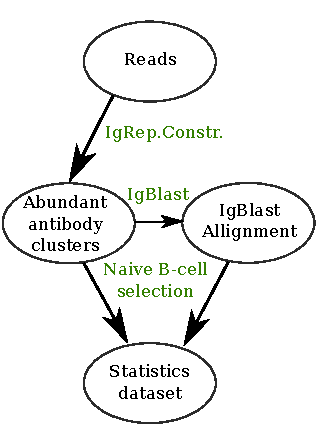
\includegraphics[width=120pt]{Pictures/downsampling.pdf}
      \end{figure}
    \end{column}
  \end{columns}
  }
\end{frame}

\begin{frame}{Cleavage and specific gene segments: \texttt{V}-genes}
 \begin{figure}[h]
  \begin{minipage}[h]{0.49\linewidth}
    \center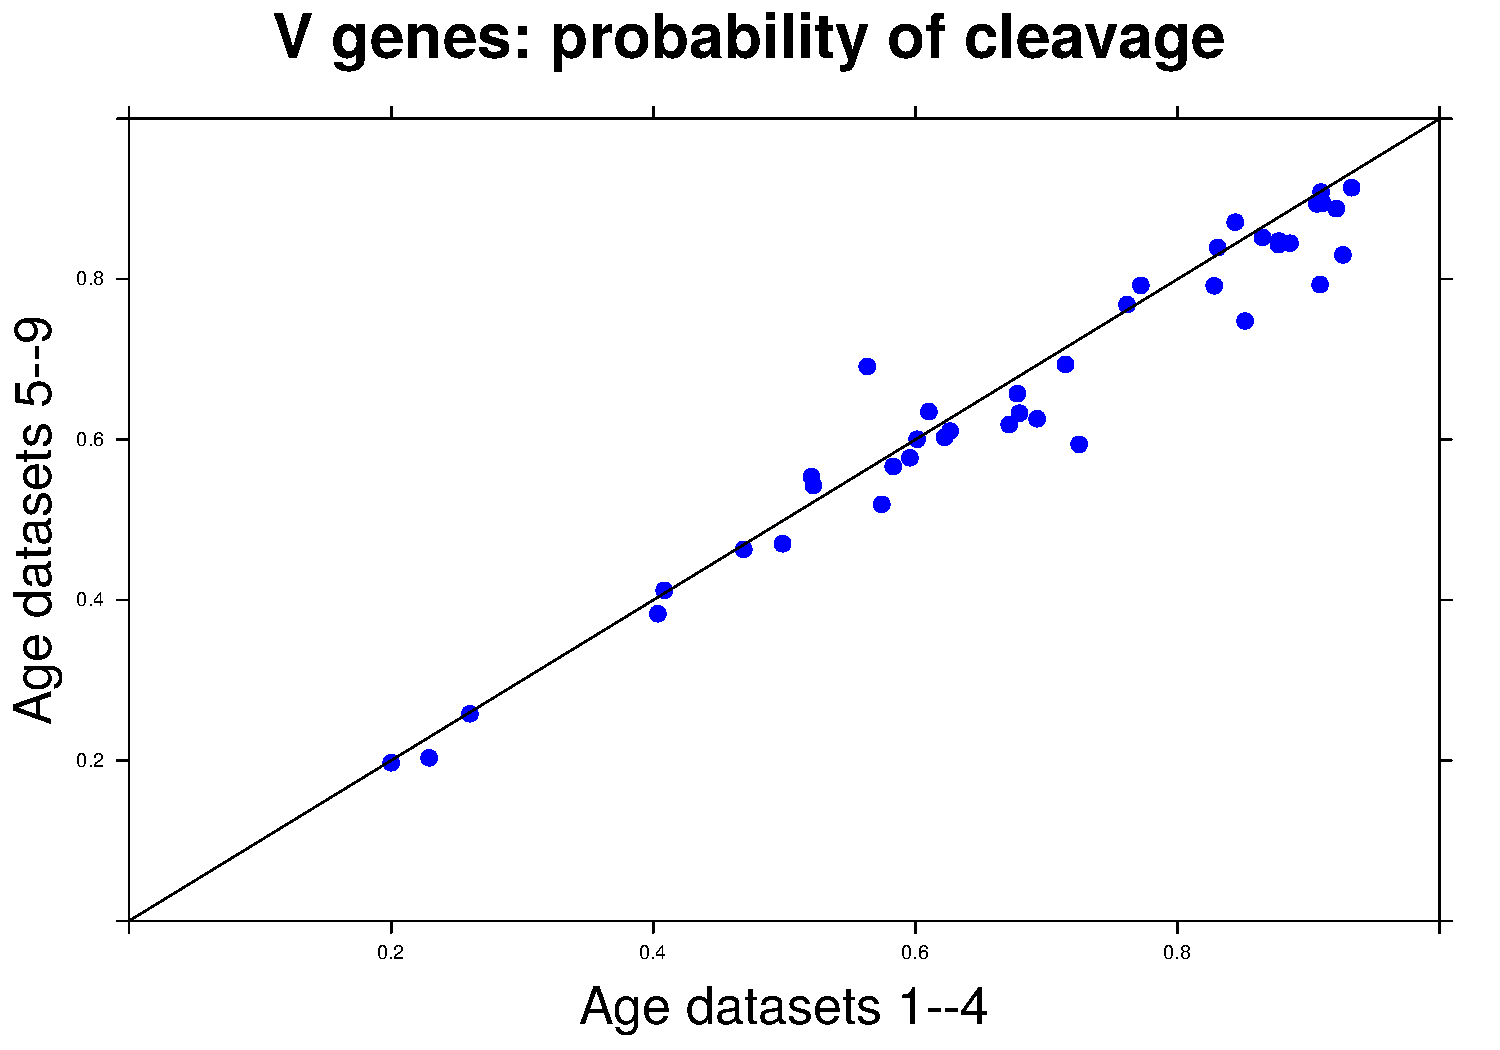
\includegraphics[width=150pt]{Vgen_cleavage_age.pdf}
    \caption{\footnotesize{\texttt{Age} datasets. The point --- is the gene. Pearson correlation is $0.98$.}} 
  \end{minipage}
  \hfill
  \begin{minipage}[h]{0.49\linewidth}
   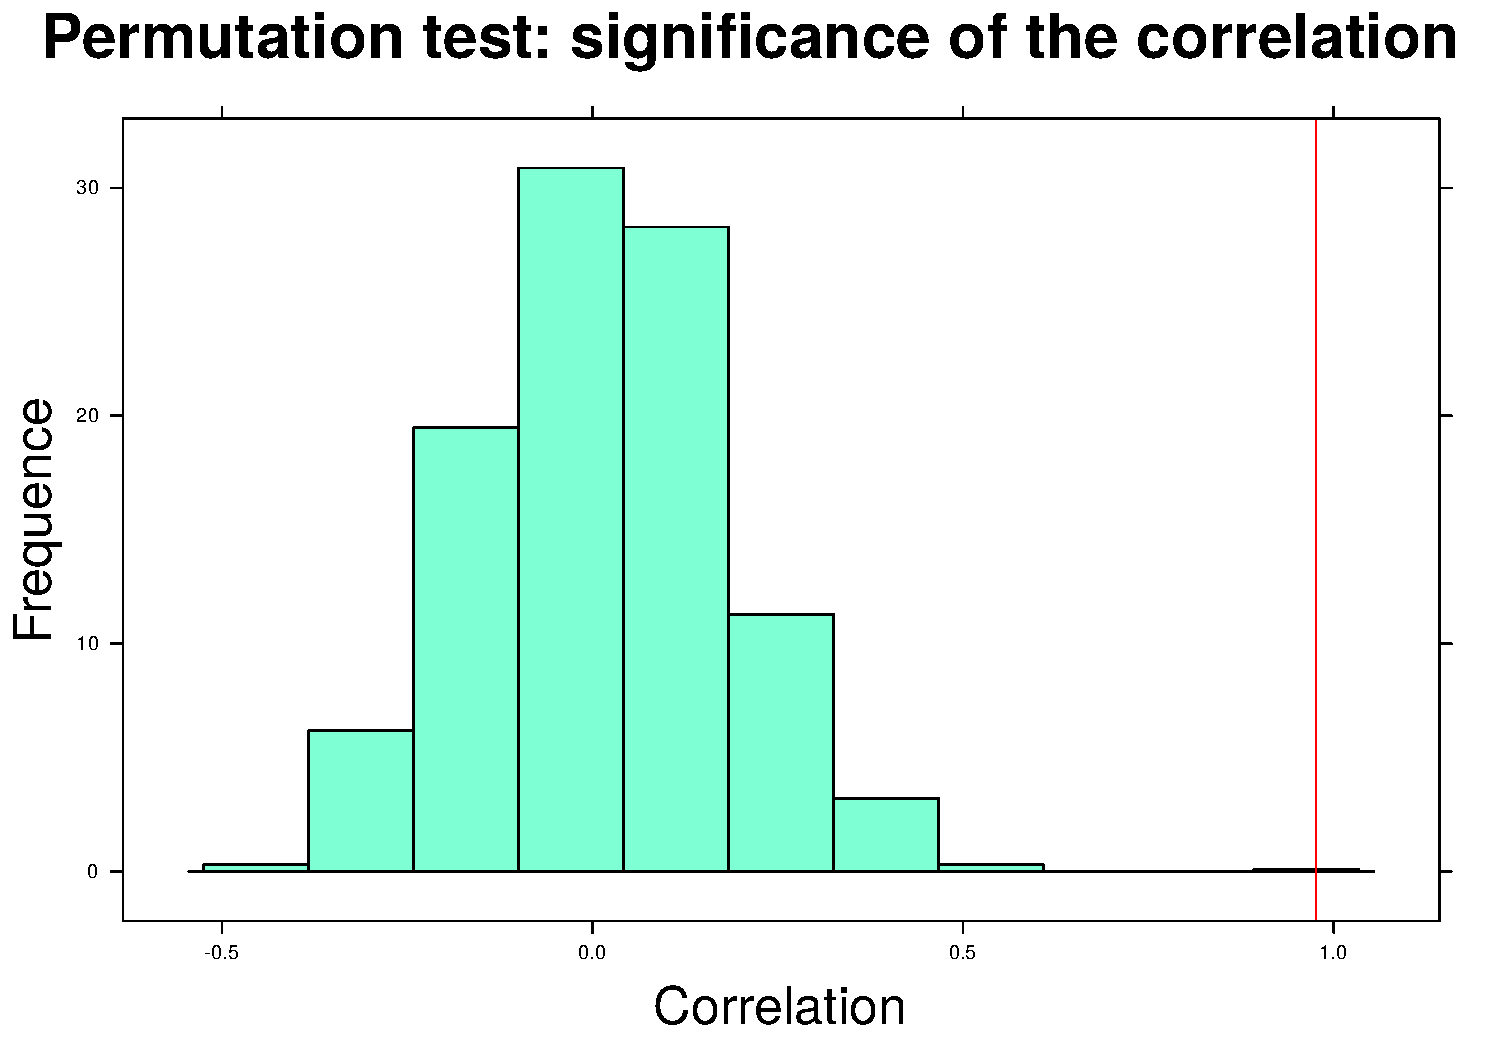
\includegraphics[width=150pt]{Vgen_cleavage_age_correlation.pdf}
    \caption{\footnotesize{Histogram of statistics of permutation test that shows the significance of Pearson correlation.}} 
  \end{minipage}
 \end{figure}
 \pause
 {\color{blue} Hence reads in the dataset are dependent standard pooled $Z$-test for equal propotions is not applicable.}
 
% textbf{Remark:} No obvious way to clusterize $V$-genes effectively due the connection.
\end{frame}

%\begin{frame}{Further goals to clusterize genes}
%  It is reasonable to seek a way to clusterize $V$-genes by
%  \begin{itemize}
%    \item \textit{palindromes} length;
%    \item \texttt{GC}-content;
%    \item different type of genes (\texttt{V} vs \texttt{J} \textit{etc\ldots}).
%  \end{itemize}
%\end{frame}

\section{Two types of palindromes}
\begin{frame}{Two types of palindromes}
  If a \textit{cleavage} took place, then no {\color{blue} ``biological''} \textit{palindrome} can happen. 
  
  \vspace{1mm}
  An {\color{blue} ``accidental''} \textit{palindrome} can still happen due to the \textit{non-genomic insertions}.
  
 \begin{figure}[h]
   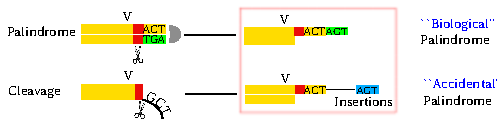
\includegraphics[width=300pt]{Pictures/two_types_palindromes.pdf}
 \end{figure}
\end{frame}

\begin{frame}{Two types of palindromes}
  \begin{itemize}
    \item The simplest model is that any nucletide $\xi$ in the sequence is distributed \textbf{uniformly}:
    \begin{gather*}
      \mathbb P(\xi = x) = \frac{1}{4} \, \mbox{ where } x \in \{'A', 'C', 'G','T'\}.
    \end{gather*}
    \item In that model the length $\eta$ of an ``accidental'' palindrome has $\mathrm{Geom}(3/4)$ distribution, so
    \begin{gather*}
      \mathbb P(\eta = n) = \frac{3}{4^{n+1}} \, \mbox { for all } n \in \mathbb N_0.
    \end{gather*}
  \end{itemize}
\end{frame}

\begin{frame}{Two types of palindromes}
  Emperical (\texttt{Age}-datasets) and $\mathrm{Geom}(3/4)$ distribution in $\log$ scale:
 \begin{figure}[h]
  \begin{minipage}[h]{0.49\linewidth}
    \center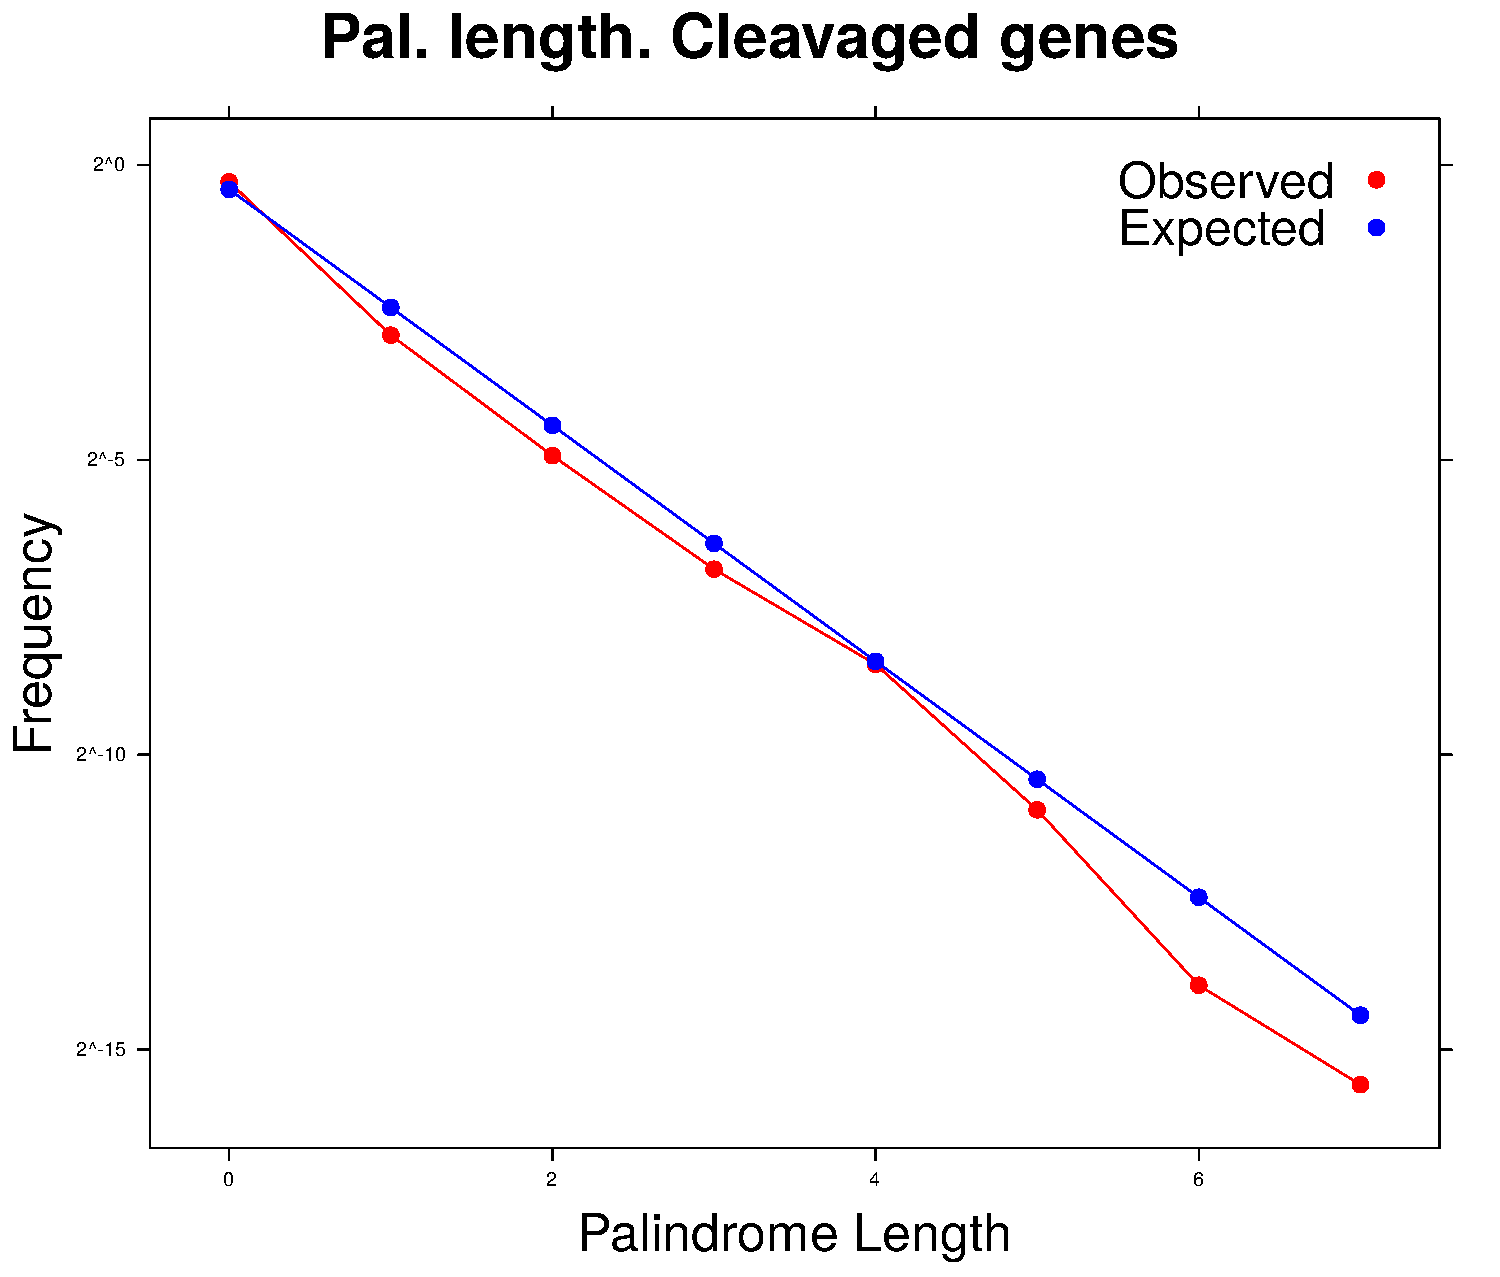
\includegraphics[width=150pt]{distr_pal_len_cl.pdf}
    \caption{\footnotesize{The $\mathrm{mean}$  of length is $0.33$.}}
  \end{minipage}
  \hfill
  \begin{minipage}[h]{0.49\linewidth}
   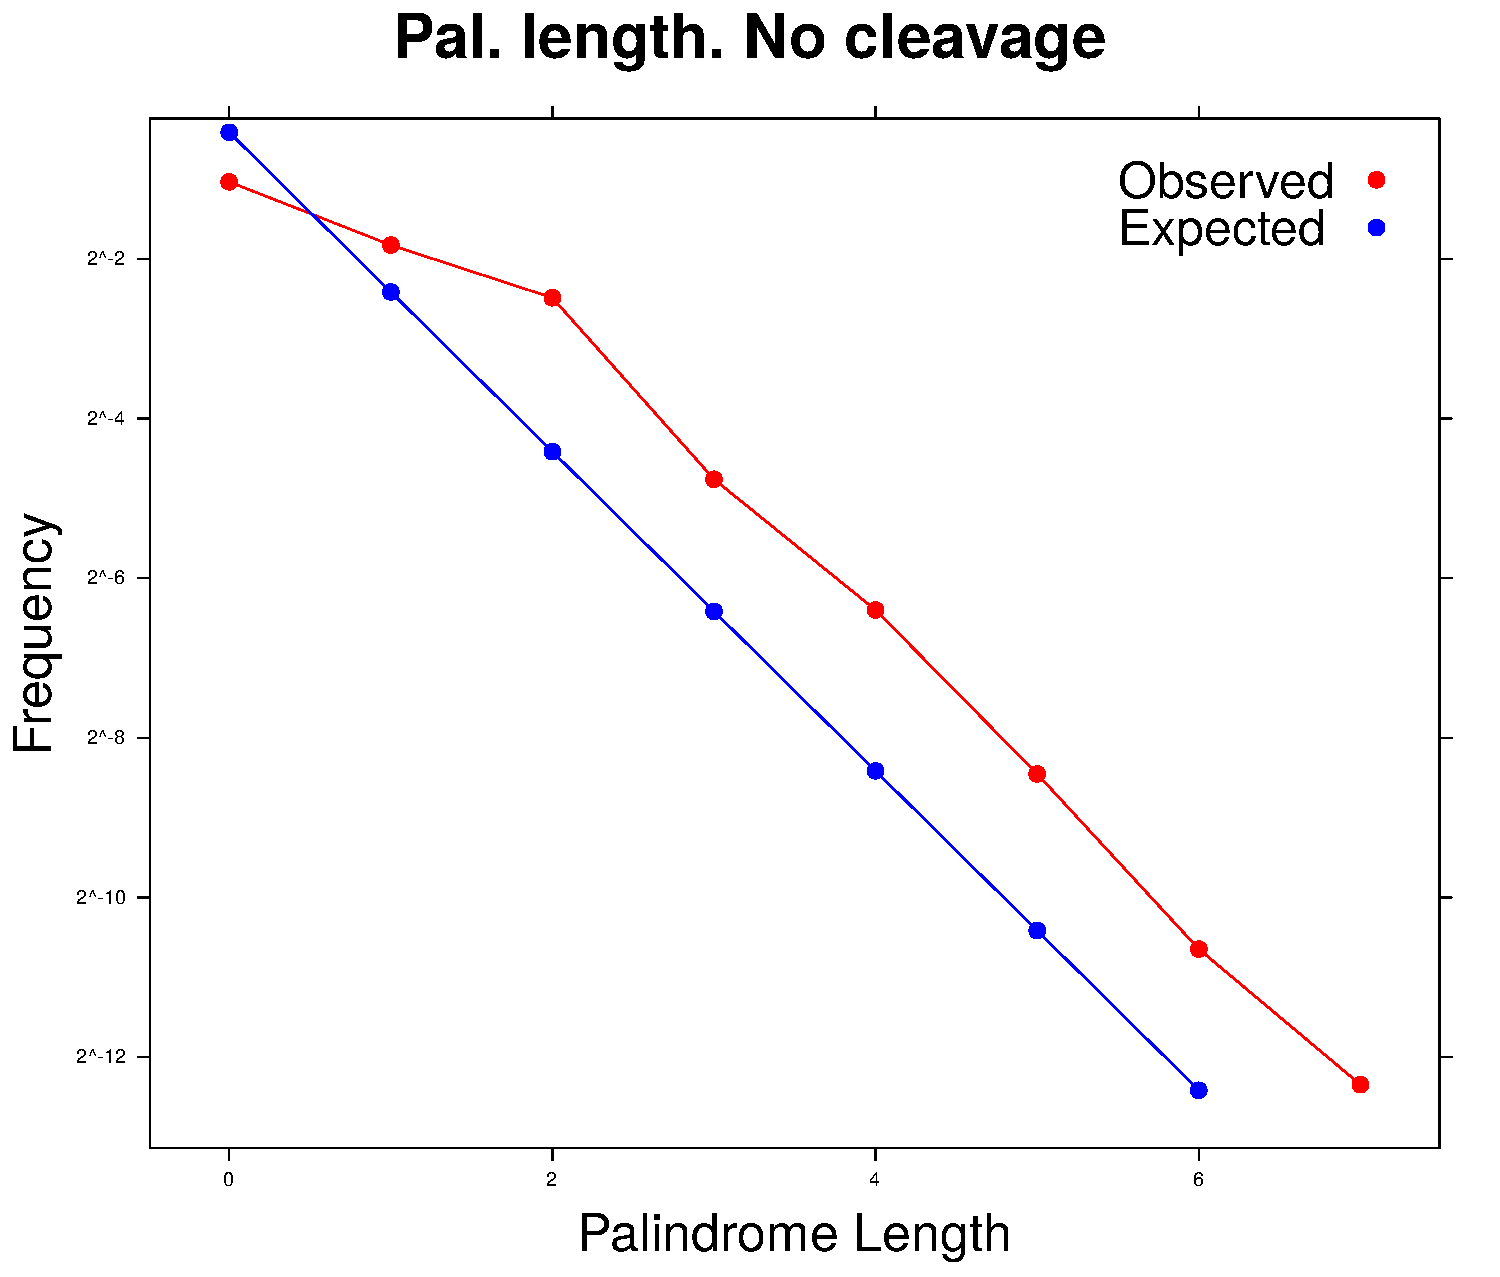
\includegraphics[width=150pt]{distr_pal_len_nocl.pdf}
   \caption{\footnotesize{The $\mathrm{mean}$ of length is $0.82$.}} 
  \end{minipage}
 \end{figure}
 
 \pause
 {\color{blue} Hence reads in the dataset are dependent goodness-of-fit $\chi^2$-test is not applicable. }
\end{frame}


\begin{frame}{Next steps}
  \begin{itemize}
    \item To find out the distribution of ``biological'' palindrome length.
    \item To construct more adequate model for nucleotide distribution.
  \end{itemize}
\end{frame}

%\section{}
%\begin{frame}{Next steps}
%  To sum up let's revisit main important questions:
%  \begin{itemize}
%    \item What is the distribution of the nucleotides?
%    \item What events are correlated strongly / weakly with each other?
%    \item How to distinguish ``biological'' and ``accidental'' events?
%  \end{itemize}
%  \bigskip
%  Also checking whether the model advised in the \href{http://www.pnas.org/content/109/40/16161.full}{%Statistical inference of the generation probability of \texttt{T}-cell receptors from sequence repertoires (
%  article} is adequate for \texttt{B}-cells (and trying to reduce the number of the parametrs) seems to be reasonable.


%  \bigskip
%  Further analysis will be concentrated on this problems.
%\end{frame}

\begin{frame}{Summary}
  Statistical analysis of an antibody repeitore is very promising research with lots of applications. Some of them:
  \begin{itemize}
    \item Comparing antibodies repertoires.
    \item Simulation of a repertoire.
    \item Edges in clonal trees.
    \item Improvement of \texttt{IgRepertoireConstructor}.
  \end{itemize}

  \bigskip
 Our goals: 
  \begin{itemize}
    \item Construct an adequate statistical model of the \texttt{V(D)J}-recombination.
    \item Find out correlations between segments of genes.
    \item Find out correlations between various biological events, including \textit{cleavage}, \textit{palindromes} and \textit{non-genomic-insertions}.
  \end{itemize}
\end{frame}

\end{document}
